% Defense slides — structured to the FMI presentation guide (figure-led, one idea/slide).
% Build:  pdflatex slides.tex   ->  slides.pdf
\documentclass[aspectratio=169]{beamer}
\usetheme{default}
\usepackage[T1]{fontenc}
\usepackage{lmodern}
\usepackage{tikz}
\usetikzlibrary{positioning, arrows.meta}
\beamertemplatenavigationsymbolsempty
\setbeamertemplate{footline}[frame number]
\graphicspath{{figures/}}

\newcommand{\figslide}[2]{%
  \begin{frame}{#1}
    \centering
    \includegraphics[width=\linewidth,height=0.82\textheight,keepaspectratio]{#2}
  \end{frame}}

\tikzstyle{box}=[draw, rounded corners, align=center, font=\footnotesize,
                 minimum height=0.95cm, minimum width=1.9cm, fill=blue!8]
\tikzstyle{off}=[box, fill=black!6]
\tikzstyle{ar}=[-{Latex[length=2mm]}, thick]

\title{Real-Time Intrusion Detection for IoT Networks}
\subtitle{NEURAL IDS — a deep-learning NIDS on CIC-IoT-2023}
\author{Rareș Marta}
\institute{Faculty of Mathematics and Computer Science\\ Babeș-Bolyai University \\[0.4em]
           {\small Coordinator: \textit{[name]}}}
\date{2026}

\begin{document}

% ---- 1. Title -----------------------------------------------------------
\begin{frame}[plain]\titlepage\end{frame}

% ---- 2. Motivation & purpose -------------------------------------------
\begin{frame}{Motivation \& purpose}
  \textbf{Why it matters}
  \begin{itemize}
    \item Billions of IoT devices, weak security — prime targets for DDoS, Mirai, scanning.
    \item Defenders need to flag malicious traffic \emph{as it happens}, per flow.
  \end{itemize}
  \vspace{0.8em}
  \textbf{Purpose}
  \begin{itemize}
    \item A real-time intrusion-detection system that classifies network flows as
          \emph{benign} or \emph{attack} and surfaces alerts live.
    \item Delivered as a working end-to-end system — not just an offline model.
  \end{itemize}
\end{frame}

% ---- 3. Outline ---------------------------------------------------------
\begin{frame}{Outline}
  \begin{enumerate}
    \item What an IDS is
    \item Data \& model — CIC-IoT-2023
    \item System architecture
    \item Demo
    \item Results \& limitations
    \item Conclusions
  \end{enumerate}
\end{frame}

% ---- 4. What an IDS is (diagram) ---------------------------------------
\begin{frame}{What an IDS does — passive detect \& alert}
  \vspace{1.2em}
  \centering
  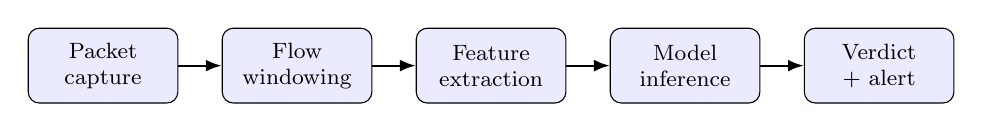
\begin{tikzpicture}[node distance=0.55cm]
    \node[box] (cap)   {Packet\\capture};
    \node[box, right=of cap]   (win)  {Flow\\windowing};
    \node[box, right=of win]   (feat) {Feature\\extraction};
    \node[box, right=of feat]  (mdl)  {Model\\inference};
    \node[box, right=of mdl]   (al)   {Verdict\\+ alert};
    \draw[ar] (cap)--(win); \draw[ar] (win)--(feat);
    \draw[ar] (feat)--(mdl); \draw[ar] (mdl)--(al);
  \end{tikzpicture}
  \vspace{1.4em}
  \begin{itemize}
    \item Observes a copy of traffic — it \emph{detects and alerts}, it does not block.
    \item Each 10-packet window between two hosts → 25 features → a calibrated verdict.
  \end{itemize}
\end{frame}

% ---- 5. Dataset ---------------------------------------------------------
\begin{frame}{The dataset: CIC-IoT-2023}
  \centering
  {\large\textbf{Canadian Institute for Cybersecurity\\ University of New Brunswick \textnormal{(2023)}}}\par
  \vspace{1.2em}
  \begin{itemize}
    \item 46.7M labelled flows · 105 real IoT devices · smart-home testbed
    \item 33 attacks across 7 families · 39-feature public CSV (packet/flow metadata)
    \item \textbf{Caveat flagged:} per-class packet windows make count features a
          near-label proxy — treated as leakage, not signal.
  \end{itemize}
\end{frame}

% ---- 6. Data processing -------------------------------------------------
\figslide{Cleaning 46.7M rows — dedup before sampling}{ingest_waterfall.png}

% ---- 7. Separability ----------------------------------------------------
\figslide{Feature separability — floods easy, web overlaps benign}{box_rate_by_family.png}

% ---- 8-10. Results ------------------------------------------------------
\figslide{Binary gate — the primary task (test set)}{confusion_2class.png}
\figslide{8-class: application-layer attacks collapse}{per_class_f1_8class.png}
\figslide{Positioning — comparable results only}{macro_f1_comparison_8class.png}

% ---- 11. Architecture (diagram) ----------------------------------------
\begin{frame}{System architecture}
  \vspace{0.6em}
  \centering
  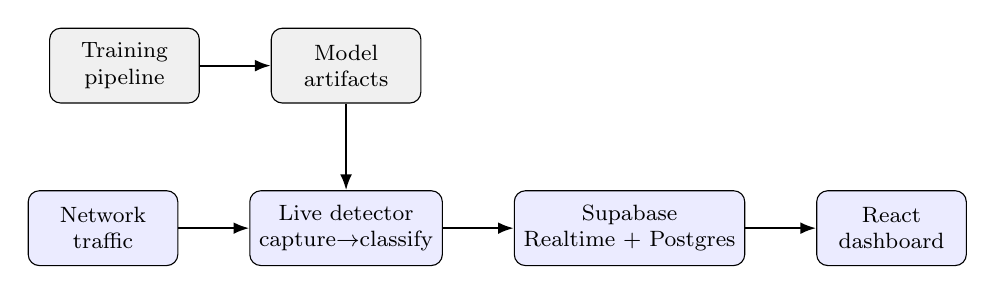
\begin{tikzpicture}[node distance=0.7cm and 0.9cm]
    % offline row
    \node[off] (train) {Training\\pipeline};
    \node[off, right=of train] (art) {Model\\artifacts};
    % online row
    \node[box, below=1.1cm of art] (det) {Live detector\\capture$\to$classify};
    \node[box, left=of det]  (traf) {Network\\traffic};
    \node[box, right=of det] (sup)  {Supabase\\Realtime + Postgres};
    \node[box, right=of sup] (dash) {React\\dashboard};
    \draw[ar] (train)--(art);
    \draw[ar] (art)--(det);
    \draw[ar] (traf)--(det);
    \draw[ar] (det)--(sup);
    \draw[ar] (sup)--(dash);
  \end{tikzpicture}
  \vspace{0.8em}
  \begin{itemize}\footnotesize
    \item Offline training emits artifacts; the live detector loads them and serves verdicts.
    \item Flows stream ephemerally over Realtime; incidents \& stats persist in Postgres.
  \end{itemize}
\end{frame}

% ---- 12. Technologies ---------------------------------------------------
\begin{frame}{Technologies}
  \centering\renewcommand{\arraystretch}{1.3}
  \begin{tabular}{ll}
    \textbf{Layer} & \textbf{Tooling}\\ \hline
    Model            & PyTorch MLP · scikit-learn (RF, RobustScaler)\\
    Data pipeline    & Polars · Apache Parquet\\
    Flow extraction  & dpkt — custom CIC-window extractor\\
    Detector service & FastAPI · Uvicorn\\
    Backplane        & Supabase (Postgres + Realtime)\\
    Dashboard        & React · Vite · Vercel\\
    Live sensor      & DigitalOcean droplet (Docker)\\
  \end{tabular}
\end{frame}

% ---- 13. Demo -----------------------------------------------------------
\begin{frame}{\textbf{Demo} — live monitoring}
  \centering
  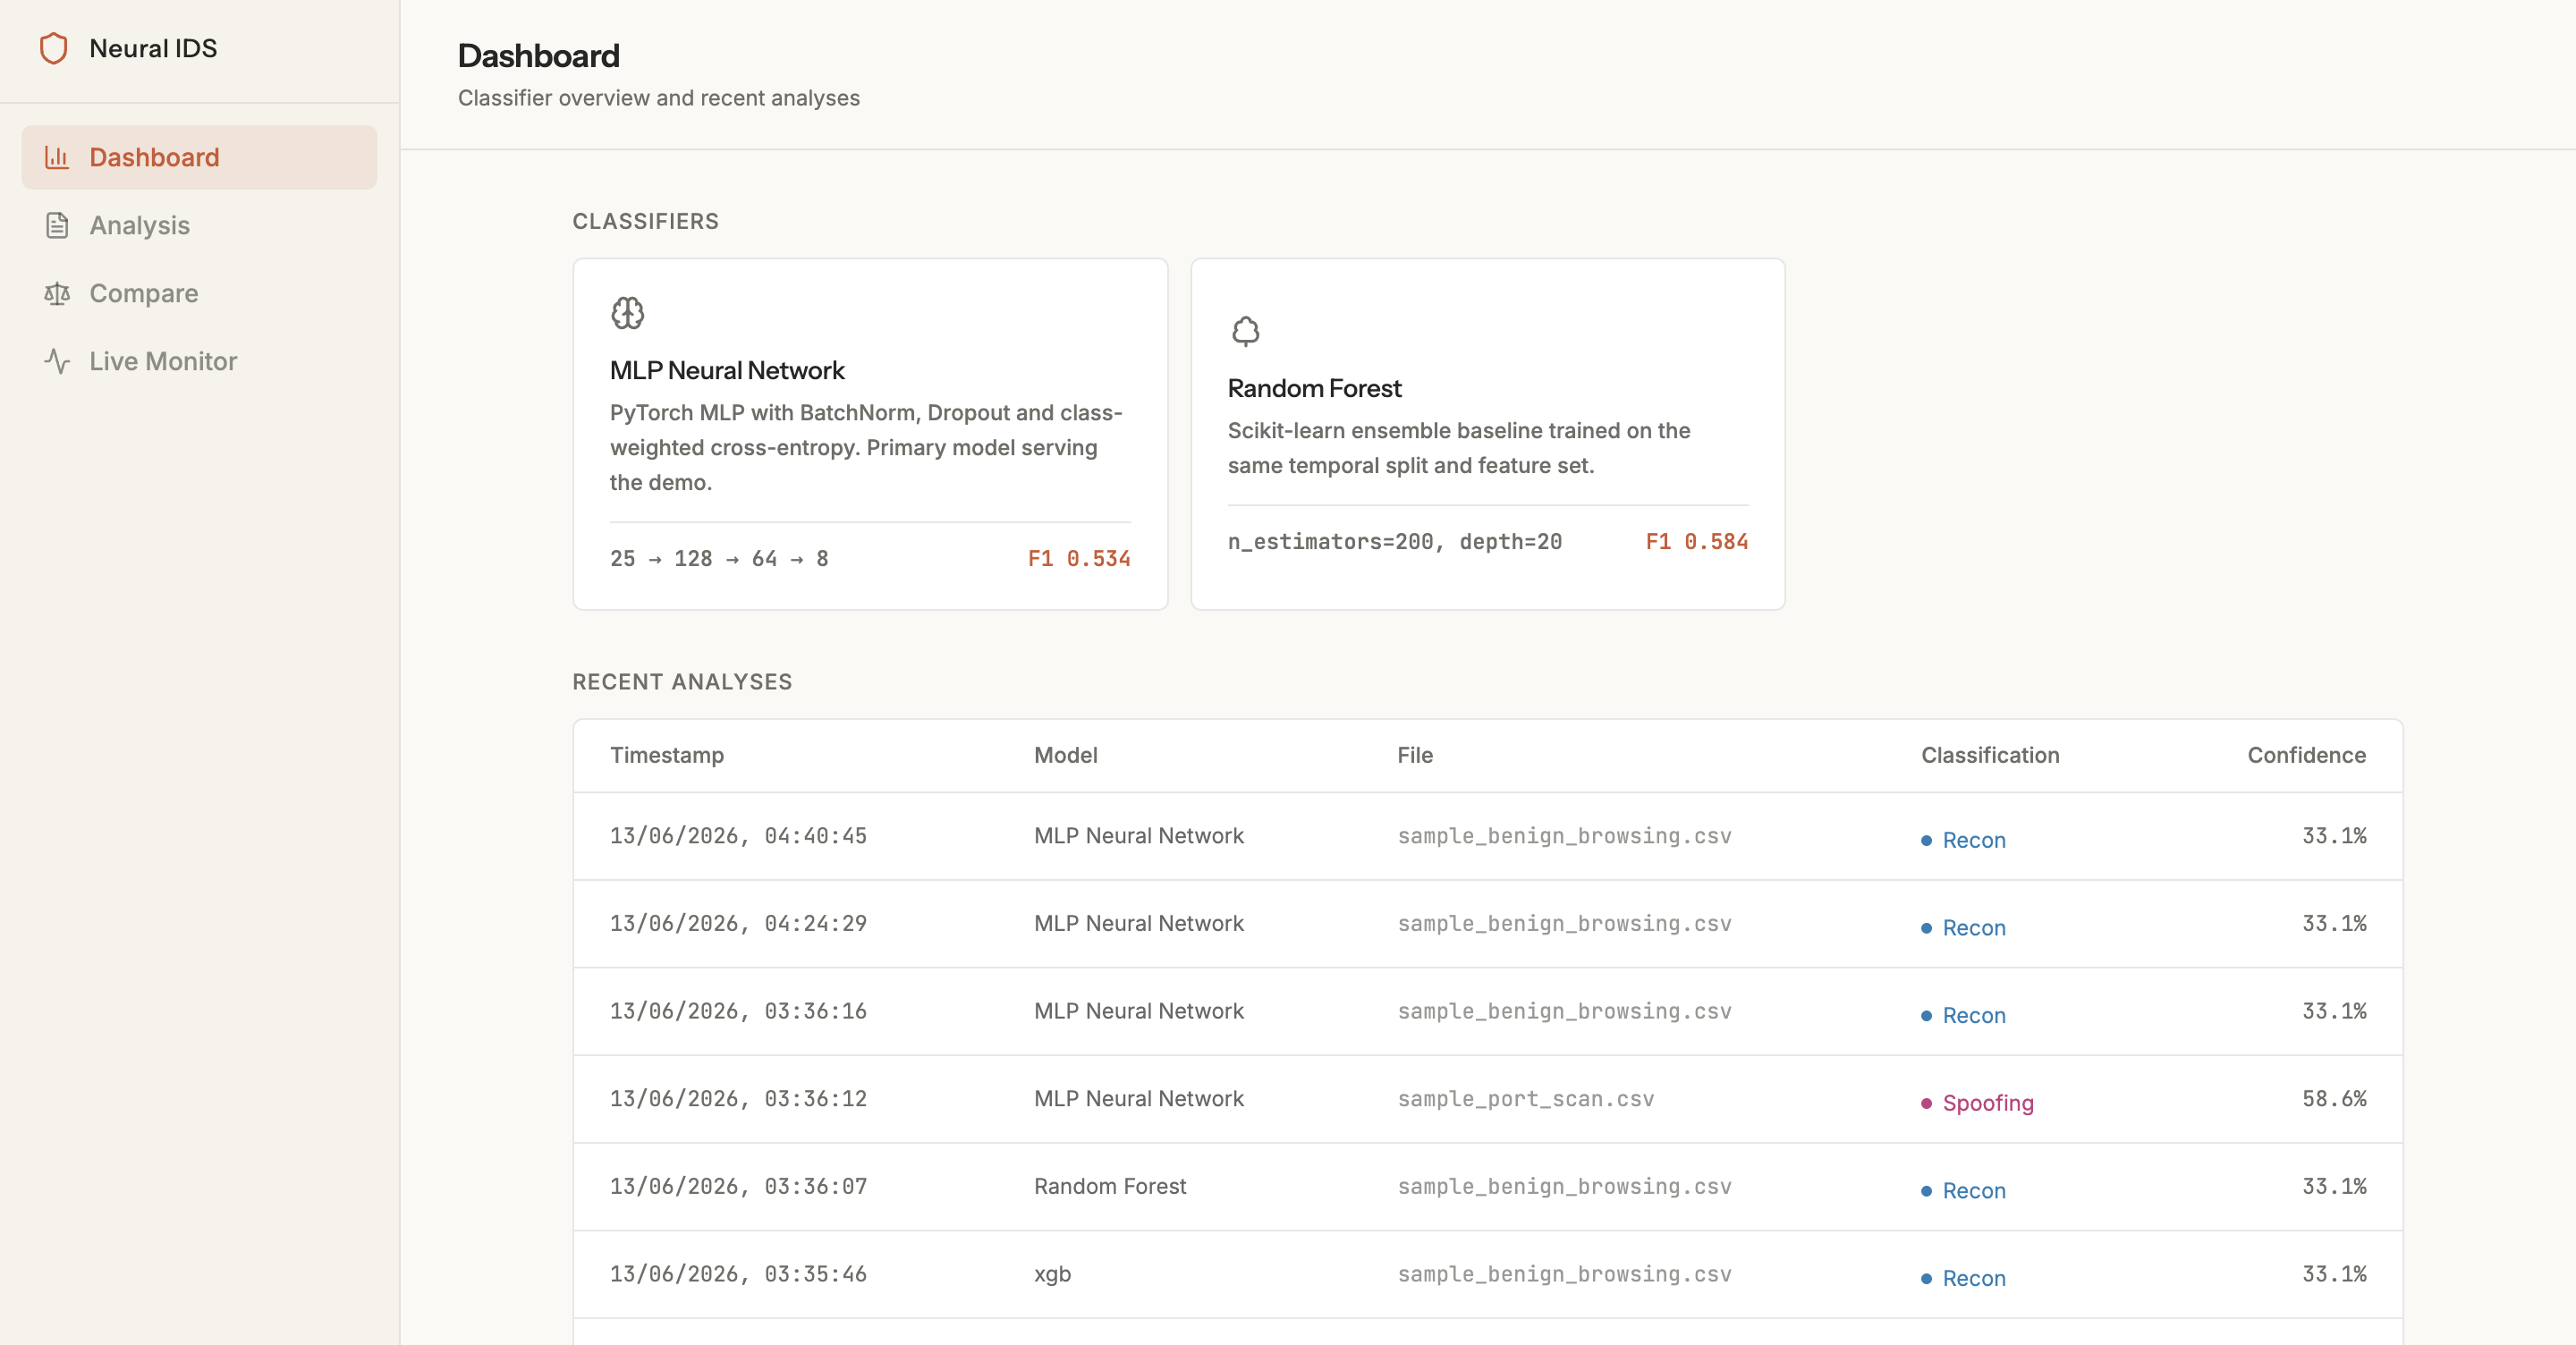
\includegraphics[width=\linewidth,height=0.66\textheight,keepaspectratio]{app_dashboard_v2.png}\\[0.4em]
  {\footnotesize Scrolling flow stream · click a flow for detail · live traffic-rate chart ·
   trigger an attack and watch it flag.}
\end{frame}

% ---- 14. Testing --------------------------------------------------------
\begin{frame}{Testing — acceptance}
  End-to-end on captures whose correct labels are known in advance:
  \begin{itemize}
    \item Benign browsing → \textbf{98\% Benign} (passes the 95\% bar)
    \item SYN flood → \textbf{100\% Attack}, mean confidence 99.6\%, family = DoS
    \item Port scan → family = \textbf{Recon}
  \end{itemize}
  \vspace{0.6em}
  In-distribution the binary gate is reliable: \textbf{MLP false-alarm rate 1.77\%}.
\end{frame}

% ---- 15. Limitation -----------------------------------------------------
\begin{frame}{Limitation — out-of-distribution traffic}
  \centering
  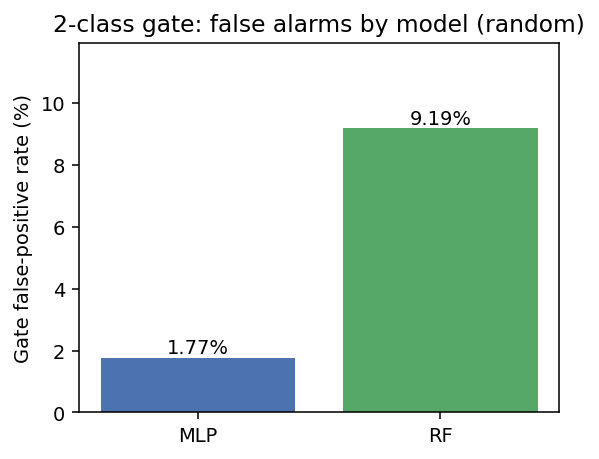
\includegraphics[width=\linewidth,height=0.52\textheight,keepaspectratio]{gate_fpr_by_model.png}\\[0.4em]
  \begin{itemize}\footnotesize
    \item In-distribution the gate over-flags only 1.77\% of benign flows.
    \item On \emph{real} internet traffic it over-flags heavily — the model's ``Benign''
          was learned from smart-home IoT devices, a different distribution (domain shift).
  \end{itemize}
\end{frame}

% ---- 16. Conclusions ----------------------------------------------------
\begin{frame}{Conclusions \& future work}
  \textbf{Delivered}
  \begin{itemize}\footnotesize
    \item A defensible MLP baseline with tree comparison on CIC-IoT-2023.
    \item A working live, streaming IDS: capture $\to$ classify $\to$ dashboard.
  \end{itemize}
  \textbf{Limitations}
  \begin{itemize}\footnotesize
    \item Out-of-distribution over-flagging (domain shift); dataset windowing leakage;
          transport-only features miss web attacks; optimistic random split.
  \end{itemize}
  \textbf{Future work}
  \begin{itemize}\footnotesize
    \item Leakage-aware retraining; fine-tune on representative traffic;
          source allow-listing / baselining; line-rate deployment.
  \end{itemize}
\end{frame}

\end{document}
